\documentclass[12pt]{article}
\usepackage[utf8]{inputenc}
\usepackage{fontspec}
\setmainfont{Times New Roman}
\usepackage{tikz}
\usepackage{amsmath}
\usepackage{indentfirst}
\usepackage{graphicx}
\usepackage{subfigure}
\usepackage{float} 
\usepackage{algorithm}
\usepackage{algorithmic}
\setlength{\parindent}{2em}
\usepackage{booktabs}
\usepackage{multirow}
\usepackage{geometry}
\usepackage{fancyhdr}
\pagestyle{fancy}
\fancyhf{}
\usepackage{xeCJK}
\usepackage{mathrsfs}
\usepackage{amsfonts,amssymb}
\usepackage{pdfpages}
\usepackage{bm}

\newcommand{\tr}{\bm{tr}}
\newcommand{\pd}{\frac{\partial}{\partial t}}
\lhead{ENGG1320 Group Project-Algorithm}
\rhead{Motion Capture}
\geometry{a4paper,scale=0.82}

\begin{document}
\noindent
    Created by He Entong
    \tableofcontents
    \newpage
    \section{Introduction}
    \subsection{Project Detail}
    This article is used for ENGG1320 group project: AI Coaching System. We introduced a method to calculate the limb actions of basketball players with wearable device (bracelet integrated with gyroscope, accelerometer and velocity detector and action-tracing gloves) and use machine learning to generate feedback for users.
    \subsection{Algorithm Framework}
    \begin{center}
    \includegraphics[width = \linewidth]{Algorithm Framework_1.png}
    \end{center}
    \section{Kalman Filter (Only for Hardware Not Integrated with A Filter)}
    Our model requires Bayesian model to build up the detection. Thus we apply Kalman filter on the dataset. The following gives a brief derivation.
    \subsection{Derivation}
    Two possible noise are the white noise $w_k \sim N(0, \sigma_{w_k}^2)$ and measurement noise $v_k$. Then for real data and data measured, 
    \begin{equation}
        x_{k+1} = \Phi x_k + w_k~~~~z_{k} = Hx_k + v_k
    \end{equation}
    Assume for data estimation, the prior prediction is $\hat x_k'$, and actual estimation is $\hat x_k$. Estimation bias is $e_k = x_k - \hat x_k$, and one assumption is that prior model bias is proportional to measurement bias, i.e.
    \begin{equation}
        \hat x_k - \hat x_k' = K_k(z_k - H\hat x_k')
    \end{equation}
    where $K_k$ is the Kalman gain. The filter tends to maximize the sum of variance of estimation bias. We first consider bias covariance matrix
    \begin{equation}
    \begin{aligned}
        E(e_ke_k^T) = P_k &= E[(x_k - \hat x_k)(x_k - \hat x_k)^T] \\
        &E[(x_k - \hat x_k' - K_kz_k + K_kH\hat x_k)(x_k - \hat x_k' - K_kz_k + K_kH\hat x_k)^T] \\
        &= (I - K_kH)E[(x_k - \hat x_k')(x_k - \hat x_k')^T](I-K_kH)^T + K_kE(v_kv_k^T)K_k^T \\
    \end{aligned}
    \end{equation}
    Define $P_k' = E[(x_k - \hat x_k')(x_k - \hat x_k')^T] = E(e_k'e_k'^T), E(v_kv_k^T) = R$ as the prior covariance matrix. Then
    \begin{equation}
        P_k = (I-K_kH)P_k'(I-K_kH)^T + K_kRK_k^T
    \end{equation}
    The model tends to minimize the variance of estimation bias (trace of covariance matrix), according to which coefficient $K_k$ is determined, that is
    \begin{equation}
    \begin{aligned}
        &\arg \min_{K_k} \tr (P_k) \rightarrow \frac{\partial}{\partial K_k}\tr(P_k) = 0\\
        &\longrightarrow  -2(H P_k')^T + 2K_k(HP_k' H^T + R) = 0 \\
        &\longrightarrow K_k = P_k'H^T (HP_k'H^T + R)^{-1} = K_k^{*}
    \end{aligned}
    \end{equation}
    then
    \begin{equation}
    \begin{aligned}
        \min \tr(P_k) &= \tr (P_k') - 2\tr [K_kHP_k'] + T\left[K_k(HP_k'H+R)K_k^T\right] \bigg|_{K_k = K_k^{*}} \\
        &= (I - K_k^{*}H)P_k'
    \end{aligned}
    \end{equation}
    Then the prior prediction bias $e_{k+1}' = x_{k+1} - \hat x_{k+1}'$. Based on previous data, prior prediction can be predicted as
    \begin{equation}
        \hat x_{k+1}' = \Phi \hat x_{k}
    \end{equation}
    Thus the prior prediction bias can be calculated as follows
    \begin{equation}
    \begin{aligned}
        e_{k+1}' &= x_{k+1} - \hat x_{k+1}' \\
        &= (\Phi x_{k} + w_k) - \Phi \hat x_{k} \\
        &= \Phi e_k + w_k
    \end{aligned}
    \end{equation}
    Notice that the bias and noise are mutually independent, hence the prior prediction bias matrix
    \begin{equation}
    \begin{aligned}
        P_{k+1}' &= E(e_{k+1}'e_{k+1}^T) \\
        &= E \left[(\Phi e_k + w_k)(\Phi e_k + w_k)^T \right] \\
        &= \Phi E(e_ke_k^T) \Phi^T + E(w_kw_k^T) = \Phi P_k \Phi^T + Q_w
    \end{aligned}
    \end{equation}
    \subsection{Loop Procedure}
    \includegraphics[width = 0.9\linewidth]{Kalman Loop.png} \par
    \begin{algorithm}[H]
        \label{KalmanLoop}
        \caption{Kalman Filter}
        \begin{algorithmic}
            \REQUIRE{sampling period $T_s$, initial state $P_0'$}
            \WHILE{$k \in T_s$}
            \STATE{Kalman Gain: $K_k = P_k'H^T(HP_k'H^T + R)^{-1}$}
            \STATE{Update Estimate: $\hat x_k = \hat x_k' + K_k(z_k - H\hat x_k')$}
            \STATE{Update Covariance: $P_k = (I - K_kH)P_k'$}
            \STATE{Project to Next Loop:  \begin{gather}
                \hat x_{k+1}' = \Phi \hat x_k \notag \\
                P_{k+1} = \Phi P_k \Phi^T + Q_w \notag
            \end{gather}}
            \ENDWHILE
        \end{algorithmic}
    \end{algorithm}
    \section{Physical Model}
    The following is the physical model to be applied in the motion detection algorithm. Physical quantities we require include the body velocity $v_b$, acceleration $a_b$, limb angular velocity $\omega_b$ and attitude angles (roll angle $\gamma$, pitch angle $\theta$).
    \subsection{Kinematic Equation}
    We first consider kinematic equation in limb movement. Acceleration $a_b$ gives
    \begin{equation}
    \begin{aligned}
        a_b &= \frac{\partial}{\partial t}{v_b} = \frac{\partial}{\partial t}(v_\theta \hat \theta + v_r \hat r) \\
        &= (\dot{v_\theta} + \dot{v_r}) + (v_\theta \frac{\partial \hat \theta}{\partial \theta}\frac{\partial \theta}{\partial t} + v_r \frac{\partial \hat r}{\partial \theta}\frac{\partial \theta}{\partial t}) = (\dot{v_\theta} + \dot{v_r}) + \omega(-v_\theta \hat r + v_r \hat \theta) = \dot{v_b} + \omega \times v_b
    \end{aligned}
    \end{equation}
    Accelerometer measurement $f_b$ and body acceleration $a_b$ has relationship
    \begin{equation}
        f_b = g_b + a_b
    \end{equation}
    Assume in accelerometer measurement, acceleration $a_b$ has relationship
    \begin{equation}
        \dot{a_b} = \eta a_b + w_1
    \end{equation}
    where Gaussian noise $w_1 \sim N(0, \sigma_{w_1}^2)$, and rational coefficient $\eta$ is a constant.
    \subsection{Stochastic Model}
    Assume that we combine the limb motion together to form a matrix $X_1$, where
    \begin{equation}
        X_1 = \begin{bmatrix}
            v_b \\ a_b
        \end{bmatrix}
    \end{equation}
    and it holds for time-shifting relationship as follows, where gyroscope zero shift $w_g$ has standard deviation $\sigma_{w_g}$.
    \begin{equation}
        \dot{X_1} = \begin{bmatrix}
            \dot{v_b} \\ \dot{a_b}
        \end{bmatrix} = \begin{bmatrix}
            a_b - \omega_b \times v_b + w_g\\
            \eta a_b + w_1
        \end{bmatrix} = \begin{bmatrix}
            -[\omega_b]_{\times} & I_3 \\
            0_3 & \eta I 
        \end{bmatrix}X_1+ \begin{bmatrix}
            w_g \\ w_1
        \end{bmatrix} = A_1X_1 + W_1
    \end{equation}
    During sampling period $T_s \in \mathcal{T}$, we have state transition equation
    \begin{equation}
    \begin{aligned}
        v_b^{(k+1)} &\approx v_b^{(k)} + \dot{v_b}^{(k)} \Delta t \rightarrow v_b^{(k+1)} \approx \left( I - [\omega_b]_{\times} T_s + R_a^v\right) v_b^{(k)} + w_g T_s
        \\a_b^{(k+1)} &\approx a_b^{(k)} + \dot{a_b}^{(k)} \Delta t \rightarrow a_b^{(k+1)} \approx (I + \eta I T_s) a_b^{(k)} + w_1 T_s
    \end{aligned}
    \end{equation}
    Then the noise covariance matrix, given that the measurement and noise have no correlation, is
    \begin{equation}
        Q_1^{(k)} = \begin{bmatrix}
            Q_{w_g}^{(k)} & 0_3 \\ 0_3 & Q_{w_1}^{(k)}
        \end{bmatrix} = \begin{bmatrix}
            \sigma_{w_g}^2 T_s^2 [v_b]_\times^{(k)} \left( [v_b]_\times^{(k)} \right)^T & 0_3 \\
            0_3 & \sigma_{w_1}^2 T_s^2 I_3
        \end{bmatrix}
    \end{equation}
    Assume the noise can be neglected in the iteration of dynamic system, then the state equation in respect of time for $X_1$ is
    \begin{equation}
        \dot{X_1} = A_1(T_s) X_1 \rightarrow X_1^{(k+1)} = \exp \left( A_1^{(k)} T_s \right) X_1^{(k)} + W_1^{(k)}
    \end{equation}
    Zhaoying Zhou et al. (2004) developed equation
    \begin{equation}
        \begin{bmatrix}
            \dot{g_x} \\ \dot{g_y} \\ \dot{g_z} 
        \end{bmatrix} = \begin{bmatrix}
            0 & -\omega_z & \omega_y \\
            \omega_z & 0 & -\omega_x \\
            -\omega_y & \omega_x & 0 
        \end{bmatrix} \begin{bmatrix}
            g_x \\ g_y \\ g_z
        \end{bmatrix} \longrightarrow \dot{g_b} = [\omega_b]_\times g_b
    \end{equation}
    Like wise, the recursive relationship and covariance matrix can be derived as
    \begin{equation}
    \begin{aligned}
        g_b^{(k+1)} = \exp \left([\omega_b]_{\times}^{(k)} T_s \right) g_b^{(k)} + W_2^{(k)}
    \end{aligned}
    \end{equation}
    where $W_2$ is corresponding process noise. Likewise, 
    \begin{equation}
    \begin{aligned}
        g_b^{(k+1)} \approx g_b^{(k)} + \dot{g}_b^{(k)} \Delta t &= g_b^{(k)} + [\omega_b]_{\times} (g_{b~\text{real}}^{(k)} + g_{b~\text{bias}}^{(k)} + g_{b~\text{noise}}) T_s \\
        &\approx (I + [\omega_b]_{\times} T_s)g_b^{(k)} + [\omega_b]_{\times} g_{b~\text{noise}} T_s
    \end{aligned}
    \end{equation}
    Then the noise covariance equation
    \begin{equation}
        Q_2 = \sigma_{g}^2 T_s^2 [g_b]_{\times} \left( [g_b]_{\times} \right)^T
    \end{equation}
    \subsection{Measurement Model}
    Assume that the data (tri-axis velocity $v_m$ and body total acceleration $f_m$) we collect from wearable device have Gaussian noise $\nu_1 \sim N(0, \sigma_{\nu_1}), \nu_2 \sim N(0, \sigma_{\nu_2})$ respectively. Then denote the state matrix as $Y$.
    \begin{equation}
        Y = \begin{bmatrix}
            v_m \\ f_m
        \end{bmatrix} = \begin{bmatrix}
            v_b + \nu_1 \\
            a_b + g_b + \nu_2
        \end{bmatrix} = \begin{bmatrix}
            I_3 & 0_3 & 0_3 \\
            0_3 & I_3 & I_3
        \end{bmatrix} \begin{bmatrix}
            v_b \\ a_b \\ g_b
        \end{bmatrix}= H\begin{bmatrix}
            X_1 \\ g_b 
        \end{bmatrix} + \nu
    \end{equation} 
    Take the augmented state matrix $X = \begin{bmatrix}
        X_1 \\ g_b
    \end{bmatrix}$ and augmented noise matrix $W = \begin{bmatrix}
        W_1 \\ W_2
    \end{bmatrix}$, then
    \begin{gather}
        Y = HX + \nu \rightarrow Y^{(k+1)} = H^{(k)}X^{(k)} + \nu^{(k)} \\
        X^{(k+1)} = \begin{bmatrix}
            \exp \left( A_1^{(k)} T_s \right) & 0_3 \\
            0_3 & \exp \left([\omega_b]_{\times}^{(k)} T_s \right)
        \end{bmatrix} X^{(k)}
        + W^{(k)} = \Phi^{(k)} X^{(k)} + W^{(k)}
    \end{gather} 
    \begin{equation}
    Q^{(k)} = \begin{bmatrix}
        Q_1^{(k)} & 0_{6 \times 3} \\
        0_{3 \times 6} & Q_2^{(k)}
    \end{bmatrix}
    \end{equation}
    Measurement noise covariance $R$ can be calculated as
    \begin{equation}
        R^{(k)} = \nu^{(k)} \left( \nu^{(k)}\right)^T
    \end{equation}
    \subsection{Filtering Process}
    Assume that $P$ is the state prediction error, then the filtering process is shown as
    \begin{center}
    \includegraphics[width = 0.75\linewidth]{Model Process.png}
    \end{center}
    \begin{algorithm}[H]
        \label{KalmanLoop}
        \caption{Data Measurement Filtering}
        \begin{algorithmic}
            \REQUIRE{sampling period $T_s$, initial state $P_0'$}
            \WHILE{$k \in T_s$}
            \STATE{Update state prediction: $(X^{(k+1)})' = \Phi^{(k)}X^{(k)}$}
            \STATE{Update prediction error: $ (P^{(k+1)})' = \Phi^{(k)} P^{(k)} ( \Phi^{(k)} )^T + Q^{(k)}$}
            \STATE{Update Kalman gain: $K^{(k+1)} = (P^{(k+1)})'(H^{(k)})^T \left( H^{(k)} (P^{(k+1)})' (H^{(k)})^T + R^{(k)} \right)^{-1}$}
            \STATE{Update state matrix: $X^{(k+1)} = (X^{(k+1)})' + K^{(k+1)} (Y^{(k+1)} - H^{(k)}(X^{(k+1)})')$}
            \STATE{Update covariance: $P^{(k+1)} = (I - K^{(k+1)} H^{(k)}) (P^{(k+1)})'$}
            \ENDWHILE
        \end{algorithmic}
    \end{algorithm}
    \subsection{From Kinematic Quantities to Attitude}
    We use Euler's angle to depict attitude of limbs.  Roll and pitch angles $(\gamma, \theta)$ can be measured by the gravitational acceleration $g_b$ we obtained from the model. Assume no yaw angle occurs, then
    \begin{equation}
    \begin{aligned}
        \bm{g}_b = \bm{Z}_{\gamma} \bm{Z}_{\theta} \bm{g}
        &= \begin{bmatrix}
            \cos \gamma & -\sin \gamma & 0 \\
            \sin \gamma & \cos \gamma & 0\\
            0 & 0 & 1
        \end{bmatrix} \begin{bmatrix}
            \cos \theta & 0 & \sin \theta \\
            0 & 1 & 0\\
            -\sin \theta & 0 & \cos \theta
        \end{bmatrix} 
        \begin{bmatrix}
            0 \\ 0 \\ -g
        \end{bmatrix} \\
        &= \begin{bmatrix}
            \sin \theta \cos \gamma \\ \sin \gamma \sin \theta \\ \cos \theta
        \end{bmatrix} g
    \end{aligned}
    \end{equation}
    Then we can come up with the attitude from the body reference frame gravitational acceleration, where
    \begin{equation}
        \left\{ \begin{aligned} &\gamma = \arctan \frac{g_{by}}{g_{bx}}  \\
            & \theta = \arctan \left( \frac{g_{by}}{\sin \gamma g_{bz}}\right) \end{aligned} \right.
    \end{equation}
\newpage 
    \section{Data Analysis}
    \subsection{Model of Users' Motion}
    We establish the state model $\bm{S}$ for motion of players. \par
    \begin{minipage}[b]{0.50\linewidth}
        \includegraphics[height=15cm]{Hook Skeleton.png}
        \end{minipage}
        \begin{minipage}[b]{0.50\linewidth}
        \includegraphics[height=15cm]{Shooting Skeleton_3.png}
        \end{minipage}
        Data considered in analysis section includes the roll angle and pitch angle of players' limbs. Upper limb angles are denoted as $(\bm{\theta}_1, \bm{\gamma}_1)$, and thigh angles are denoted as $(\bm{\theta}_2, \bm{\gamma}_2)$. Wearable devices are adjusted to two independent coordinate respectively. Average angular velocity $\bar{\bm{\omega}}$ can be measured by
        \begin{equation}
            \bar{\bm{\omega}} = \frac{1}{\sum_{T_s} \Delta t}\sum_{t \in T_s} \bm{\theta}(t)
        \end{equation}
        Assume during time period $(t_1, t_2)$, positive total acceleration is detected, then the maximum height $h$ from the ground can be measured by
        \begin{equation}
            h = \frac{1}{2} g \left( \sum_{t_1}^{t_2} \Delta t\right)^2
        \end{equation}
        Under polar coordinate, we depict the comparative position of user with the basket with $(\beta, r)$.
        Then the complete characteristic vector $\bm{S}$ is
        \begin{equation}
            \bm{S} = \begin{bmatrix}
                \bm{\theta}_1 & \bm{\gamma}_1 & \bm{\theta}_2 & \bm{\gamma}_2 & \bar{\bm{\omega}_1} & h & \beta & r
            \end{bmatrix}^T
        \end{equation}
        where
        \begin{gather}
            \bm{\theta}_1 = \begin{bmatrix}
                \theta_{\text{left upperlimb}} & \theta_{\text{right upperlimb}}
            \end{bmatrix} \\ \bm{\gamma}_1 = 
            \begin{bmatrix}
                \gamma_{\text{left upperlimb}} & \gamma_{\text{right upperlimb}}
            \end{bmatrix} \\
            \bm{\theta}_2 = \begin{bmatrix}
                \theta_{\text{left thigh}} & \theta_{\text{right thigh}}
            \end{bmatrix} \\ \bm{\gamma}_1 = 
            \begin{bmatrix}
                \gamma_{\text{left thigh}} & \gamma_{\text{right thigh}}
            \end{bmatrix}
        \end{gather}
    \subsection{Data Analysis Method: Support Vector Machine}
    The user shooting outcome can be mapped into label space $\mathcal{H}$, where
    \begin{equation}
        \mathcal{H} = \left\{ \begin{aligned}
            -&1 &\text{field goal miss} \\
            &1 &\text{field goal made}
        \end{aligned} \right.
    \end{equation}
We use Support Vector Machine to study the motions of professional athletes. To avoid non-linear dataset, radius basic function is applied as the kernel function, where
\begin{equation}
    K(x, y) = \exp \left( -\frac{||x - y ||^2}{2 \sigma^2}\right)
\end{equation}
Penalty factor $C$ is set comparatively low to achieve higher generalization. SVM training will find solution of following target
\begin{gather}
    \arg \min_{\bm{\alpha}} \frac{1}{2}\sum_{i=1}^N \sum_{j=1}^N \alpha_i \alpha_j y_i y_j K(\bm{x}_i,\bm{x}_j) - \sum_{i=1}^N \alpha_i  \notag \\ \text{s.t.}~\sum_{i=1}^N \alpha_i y_i = 0,~0 \leq \alpha_i \leq C
\end{gather}
with optimal multiplier $\bm{\alpha}^*$ obtained, the weight $\bm{w}$ and bias $b$ can be calculated
\begin{gather}
    \bm{w}^* = \sum_{i=1}^n \alpha_i^* y_i \bm{x}_i \\
    y_j(K(\bm{w}^*, \bm{x}_j) + b^*) = 1 \rightarrow b^* = y_j - \sum_{i=1}^n \alpha_i^* y_i K(\bm{x}_i, \bm{x}_j)
\end{gather}
We use sklearn library integrated in Python (prototype LIBSVM in C++) to complete the training process. Weight vector and bias will be stored in the *.m file to be used for data analysis later on. The update on the training app will include maintenance on shooting database. 
\subsection{Feedback Algorithm}
Once the weight vector and bias is studied, it can be used in giving feedback to users. Assume that the data collected from user is $\bm{S}$, then the decision-making function is
\begin{equation}
    f(\bm{S}) = sign(K(\bm{w}, \bm{S}) + b)
\end{equation}
We tend to make the inner quantity as large as possible, which increases the possibility to make field goal according to the database. Since all the physical quantities take positive values, we use an intuitive algorithm to generate the feedback: increase the parameter with positive weight, and decrease the parameter with negative weight. We take order to optimize the shooting motion. With short-distance shot (inside the free throw line), we suggest two-motion shots. So bounce height will be considered more important. By contrast, in long-distance one, we suggest one-motion shots and put more priority to upper limb and thigh attitude. Assume the threshold value for distance is $r_t$, then the following gives the graph of our optimizing order. \par \noindent
With $r < r_t$ (two-motion shot),
\begin{center}
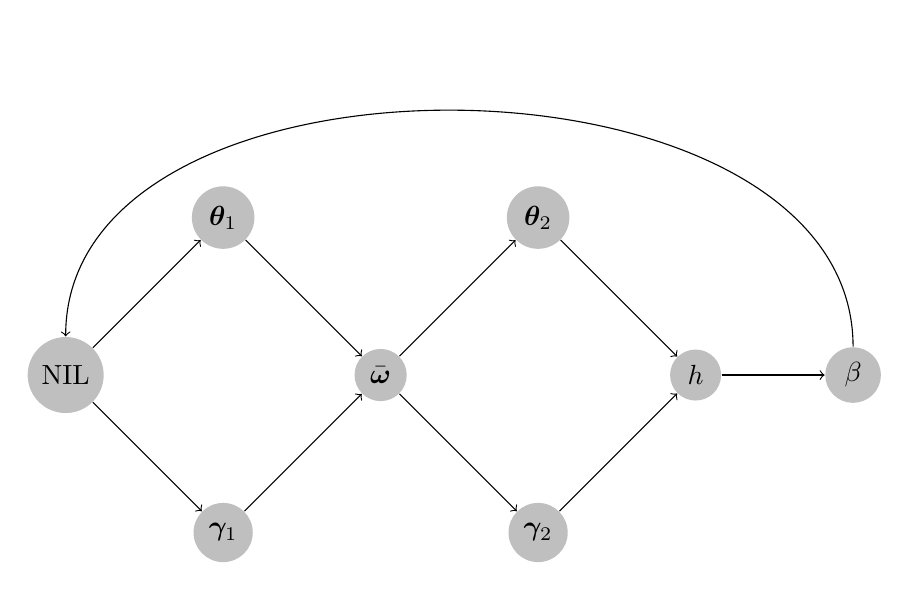
\begin{tikzpicture}
    \node[shape=circle,fill=lightgray] (a) at (0, 0) {NIL};
    \node[shape=circle,fill=lightgray] (b1) at (2, 2) {$\bm{\theta}_1$};
    \node[shape=circle, fill=lightgray] (b2) at (2,-2) {$\bm{\gamma}_1$};
    \node[shape=circle, fill=lightgray] (c) at (4,0) {$\bar{\bm{\omega}}$};
    \node[shape=circle,fill=lightgray] (d1) at (6,2) {$\bm{\theta}_2$};
    \node[shape=circle,fill=lightgray] (d2)at (6,-2) {$\bm{\gamma}_2$};
    \node[shape=circle,fill=lightgray] (e) at (8,0) {$h$};
    \node[shape=circle,fill=lightgray] (f) at (10,0) {$\beta$};
    \draw[->] (a) -- (b1);
    \draw[->] (a) -- (b2);
    \draw[->] (b1) -- (c);
    \draw[->] (b2) -- (c);
    \draw[->] (c) -- (d1);
    \draw[->] (c) -- (d2);
    \draw[->] (d1) -- (e);
    \draw[->] (d2) -- (e);
    \draw[->] (e) -- (f);
    \draw[->] (f) to [out = 90,in=90] (a);
\end{tikzpicture}
\end{center}
With $ r\geq r_t$ (one-motion shot), 
\begin{center}
    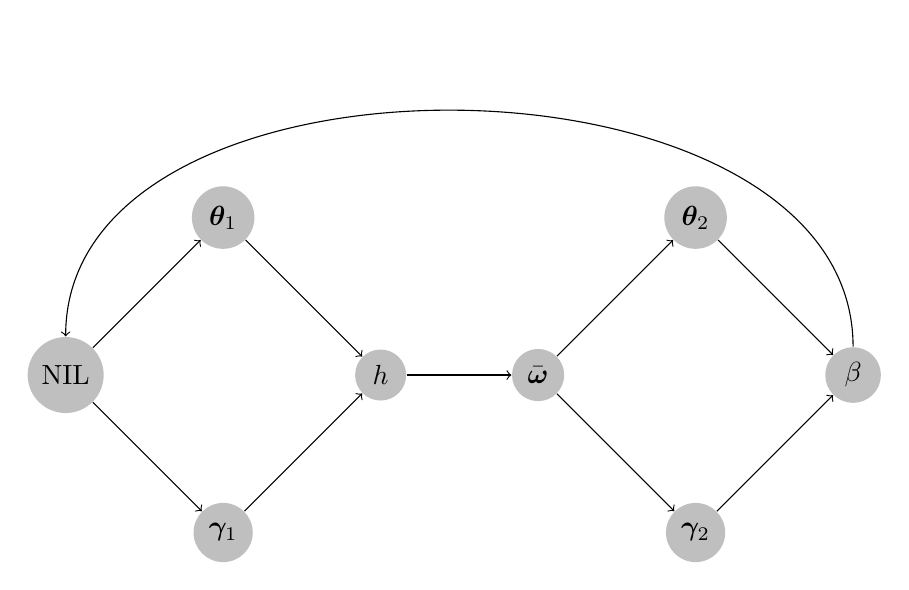
\begin{tikzpicture}
        \node[shape=circle,fill=lightgray] (a) at (0, 0) {NIL};
        \node[shape=circle,fill=lightgray] (b1) at (2, 2) {$\bm{\theta}_1$};
        \node[shape=circle, fill=lightgray] (b2) at (2,-2) {$\bm{\gamma}_1$};
        \node[shape=circle, fill=lightgray] (c) at (6,0) {$\bar{\bm{\omega}}$};
        \node[shape=circle,fill=lightgray] (d1) at (8,2) {$\bm{\theta}_2$};
        \node[shape=circle,fill=lightgray] (d2)at (8,-2) {$\bm{\gamma}_2$};
        \node[shape=circle,fill=lightgray] (e) at (4,0) {$h$};
        \node[shape=circle,fill=lightgray] (f) at (10,0) {$\beta$};
        \draw[->] (a) -- (b1);
        \draw[->] (a) -- (b2);
        \draw[->] (b1) -- (e);
        \draw[->] (b2) -- (e);
        \draw[->] (e) -- (c);
        \draw[->] (c) -- (d1);
        \draw[->] (c) -- (d2);
        \draw[->] (d1) -- (f);
        \draw[->] (d2) -- (f);
        \draw[->] (f) to [out = 90,in=90] (a);
    \end{tikzpicture}
    \end{center}
\newpage
In every feedback process, the program will search for optimization in the graph above using BFS. It continually searches for positive weight nodes and negative weight nodes, and use step size $\eta$ which is uniquely set up for each node. Every time a node $v$ is visited, its corresponding step size $\eta_v$ will be added/deduced according to its weight.\
\begin{algorithm}[H]
    \label{feedback algorithm}
    \caption{BFS($\bm{S}$)}
    \begin{algorithmic}
        \REQUIRE{priority graph $G(V, E)$}
        \STATE{intialize feedback vector $\bm{f} = \bm{0}$, starting vertex $s = G.$NIL, queue $Q$}
        \STATE{$Q.enqueue(s)$}
        \WHILE{$sign(K(\bm{w}, \bm{S} - \bm{f}) + b) \neq 1$}
        \STATE{$u \gets Q.deque$}
        \FOR{$v \in u.adj$}
        \IF{$\bm{w}.v \geq 0$}
        \STATE{$\bm{f}.v \gets \bm{f}.v + \eta_{v}$}
        \ELSE
        \STATE{$\bm{f}.v \gets \bm{f}.v -\eta_{v}$}
        \ENDIF
        \STATE{$Q.enqueue(v)$}
        \ENDFOR
        \ENDWHILE
        \RETURN{$\bm{f}$}
    \end{algorithmic}
\end{algorithm}
With the feedback vector, it is easy to generate the feedback for users literally and schematically.
\end{document}